% !TeX spellcheck = en_US
% !TEX root = ../thesis-example.tex
%
\section{Virtual projection parameters from real world camera}
\label{sec:projection-params}
To reproduce a virtual projection for the real world camera there are four 
initially unknown variables:

\begin{my_list}
	\item Position of the real world camera
	\item Rotation of the real world camera
	\item Field of View (FoV) of the camera
	\item Distance between the HMD and the real world camera
\end{my_list}

Luckily the former two are solved by the tracking solution and can be used 
directly as transformation matrix for the virtual casmera - ignoring an 
additional fixed offset from the actual controller to the camera, which is 
accounted for inside the software.
\newline
The calculation of a corresponding distance between a camera and the Vive HMD 
to control the virtual projection parameters can be solved, too: Since both 
devices are tracked, one natively and the other with a controller as 
tracking anchor, it can be calculated with the same euclidean distance as 
discussed earlier, with $C$ as camera position and $H$ as HMD position:

\eq{eq:zsort:distance}{
	Z = \sqrt{(C_X + H_X)^2 + (C_Y + H_Y)^2 + (C_Z + H_Z)^2}
}

\begin{figure}[htb]
	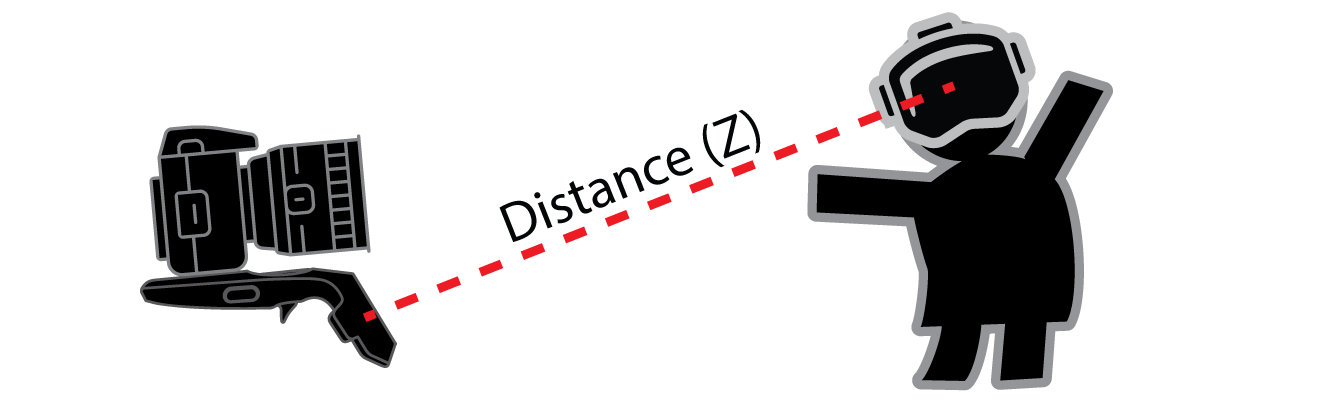
\includegraphics[width=\textwidth]{gfx/distance-z.png}
	\caption{Distance correlation between real world camera and the VR actor}
	\label{fig:projection:distance}
\end{figure}

Another important projection parameter is field of view. Most production 
cameras only declare a focal length on lenses - which makes sense in that 
context, since field of view is a constraint between sensor size and focal 
length, varying from camera object to another. Through the specification sheet 
of the camera the current field of view can be calculated inside Unity, with 
the sensor height as $S_h = 17.3mm$ and focal length as $F_l = 14mm$:

\eq{eq:zsort:fov}{
	FoV = 2*tan^{-1}\frac{S_h}{2 * F_l}
}

\eq{eq:zsort:fov:result}{
	FoV = 63.42028^\circ
}

With that we have now all projection parameters reconstructed for the virtual 
environment to generate an image that matches in relative transformation 
parameters as the real world camera would look at.